\chapter{Literature Review}\label{ch:literature}

In this chapter, some basic concepts and important knowledge are provided. These concepts are 

\section{Planetary gearbox}

Planetary gearing or epicyclic gearing is a gear system typically consisting of four parts: sun gear, planet gear, ring gear and the planet carrier.

There are several ways of input-output method such as stationary ring gear, fixed carrier or no stationary part. The gear ratio of the of the planetary gearbox could be calculated as:

\begin{equation}
	N_s\omega_s + N_r\omega_r - (N_s + N_r)\omega_c
\end{equation}

The following figure shows a typical planetary gearing system, which contains 3 planet gears.

\begin{figure}[h]
	\centering
	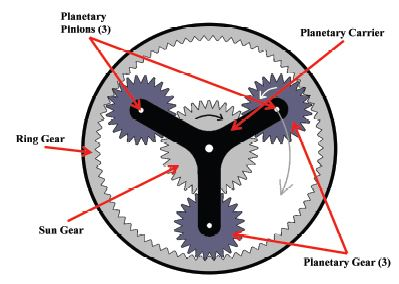
\includegraphics[width=5cm]{PGB}
	\caption{Planetary Gearbox Layout ~\cite{forrester}}
	\label{simulationfigure}
\end{figure}


The characters of planetary gearbox make it suitable for large transmission ratio, high load and split input or output circumstances. So it is widely used in wind turbines, lathes, automobiles and helicopters. 

















Previously, Nooshabadi~\cite{pa} has descried style-related thesis
requirements, Shepherd~\cite{She05} has provided \LaTeX\ templates while
other academics have discussed contents with their students.  This work
draws all the relevant information regarding thesis writing into one
document.  The present template/document is heavily influenced by
Nooshabadi and Shepherd, incorporating requirements from The Graduate
Research School~\cite{GRS14} for Higher Degree Research theses.


\section{Gear fault diagnosis}

\subsection{Vibration generated by gear}

1)	Normal operation

2)	Fault, spalls and cracks

\subsection{Diagnosis techniques}

1)	Standard Indicators

2)	wavelet

3)	Cepstrum

4)	TSA

5)	Order tracking

6)	Machine learning method


\section{Variable Speed}